\documentclass[a4paper,10pt]{article}
\usepackage[utf8]{inputenc}
\usepackage{multirow}
\usepackage{hyperref}
\usepackage{graphicx}

%opening
\title{Exploring Trade-Offs and Synergies}
\author{L. Hertzog}

\graphicspath{{./figures/}}

\begin{document}

\maketitle

\section{Background}

Data were simulated to explore the observed and modelled correlation between two response variables. The simulation involved the following steps with variations:

\begin{enumerate}
 \item Generate a (residual) correlation matrix between the response variables, the correlation coefficient was set at 0.6 for the simulations with residual correlations and at 0.01 or -0.01 for no residual correlation
 \item 100 random values were drawn for the predictor(s) from an uniform distribution (min. -2, max. 2)
 \item Linear predictors were computed for the two variables, the effect of the predictor could either be: (i) consistent, same slopes for the both response variables or (ii) divergent, slopes have opposite signs for between the two response variables
 \item Based on the correlation matrix and the linear predictors, response variables were simulated 100 times from a multivariate normal distribution (mvtnorm::rmvnorm)
 \item The observed correlation coefficient between the response variables was computed
 \item A multivariate model was fitted to the response variable using Stan and the median of the posterior draw of the correlation coefficient was computed.
 \item The observed and modelled correlation were then compared to the simulated values and three cases are defined (See table~\ref{tab:cat}): (i) extrinsic correlation: presence of observed correlation but no residual correlation from the model, all the correlation between two variables are driven by their response to a common driver, (ii) intrisic correlation: presence of both observed and residual correlation, the correlation is driven by some intrisic process between the variables or some predictors are missing from the model, (iii) appearing correlation: absence of observed correlation but presence of residual correlation, due to some confounding effect from a common driver correlation between two variables is masked.
\end{enumerate}

\begin{table}[h!]
 \caption{Different possibilities of observed and residual (after model fitting) correlations with the name given to the different outcomes.}
 \vspace*{0.5cm}
 \label{tab:cat}
 \begin{tabular}{lc|cc|}
  & & \multicolumn{2}{|c|}{Observed correlation} \\
  & & Present & Absent \\ \hline
  \multirow{2}{*}{Residual correlation} & Present & Intrisic & Appearing \\
  & Absent & Extrinsic & NA \\
 \end{tabular}

\end{table}



\section{First simulations: one predictor, two responses}

The different scenarios are schematically represented in Figure~\ref{fig:schema1}

\begin{figure}[h!]
 \caption{Schematic representation of the first batch of scenarios. X is the predictor variable which effect the two response variables Y1 and Y2, these response variables have positive correlation (+) or have virtually no correlation (0). }
 \label{fig:schema1}
 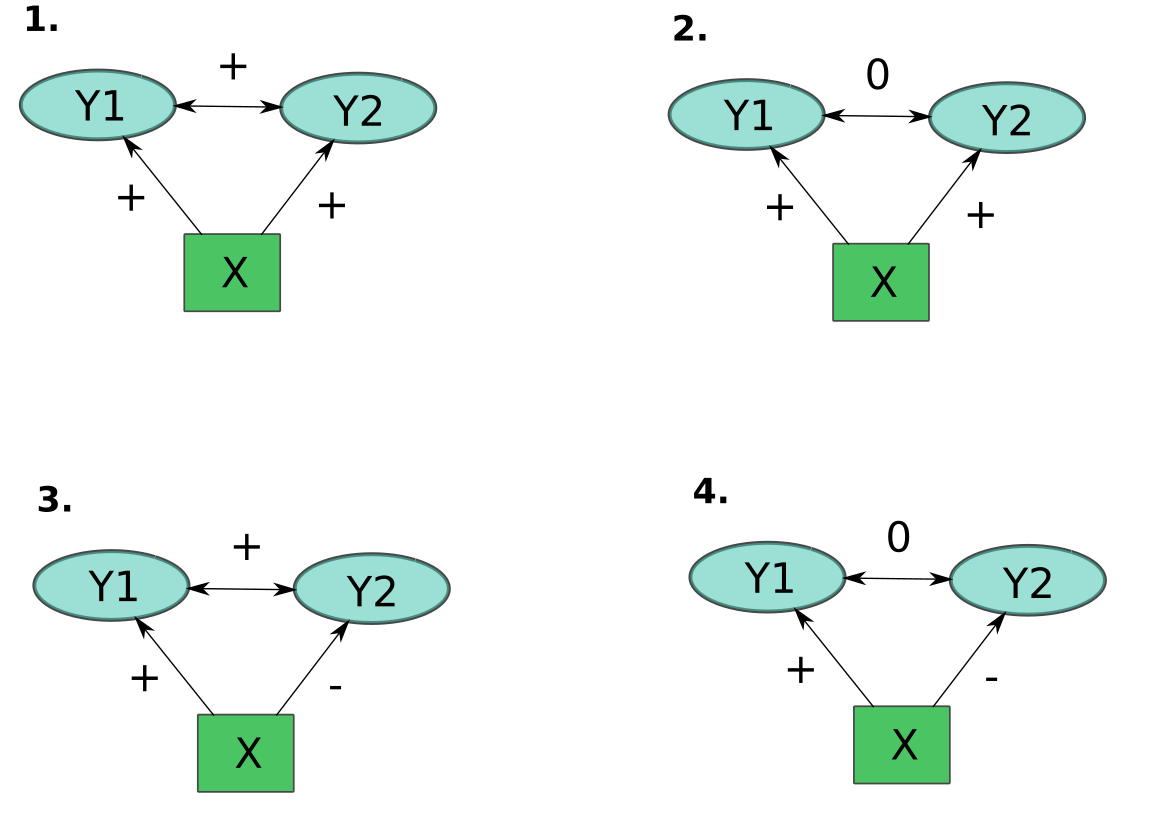
\includegraphics[width=\textwidth,keepaspectratio]{simulation1_4.png}
\end{figure}


\begin{table}[h!]
\caption{Result first simulation round}
\label{tab:res1}
 \begin{tabular}{lccr}
  Scenario ID & Predictor effect & Residual correlation & Result \\ \hline
  1 & consistent & yes (positive) & Intrisic correlation \\
  2 & consistent & no & Extrinsic correlation \\
  3 & divergent & yes (positive) & Intrisic or appearing correlation \\
  4 & divergent & no & Extrinsic correlation
 \end{tabular}
\end{table}


The result show that \textbf{extrinsic correlation} (correlation present in observed data but not after model) can be cause by: consistent response to a common driver (synergies, scenario 2) or divergent response to a common driver (trade-off, scenario 4). \textbf{Intrisic correlation} can be caused by consistent effect of a common driver together with residual correlation (scenario 1), but also with divergent effect of a common predictor and residual correlation (scenario 3). In this last case the balance between the strength of the residual correlation and the strength of the effect can also lead to \textbf{apparing correlation} (correlation that were not present in the observed data but are present in the residuals) but also to sign inversion in the correlation coefficient. This is for instance the case when there is strong residual correlation and strong effect of the predictor going in opposite direction. 

\begin{figure}
 \caption{Fitted correlation coefficient for observed data (raw correlation coefficient) and based on the model (median of the posterior draws), done for 100 repetition and for the 4 different scenarios, see Table~\ref{tab:res1}. The dashed line represent the simulated real value.}
 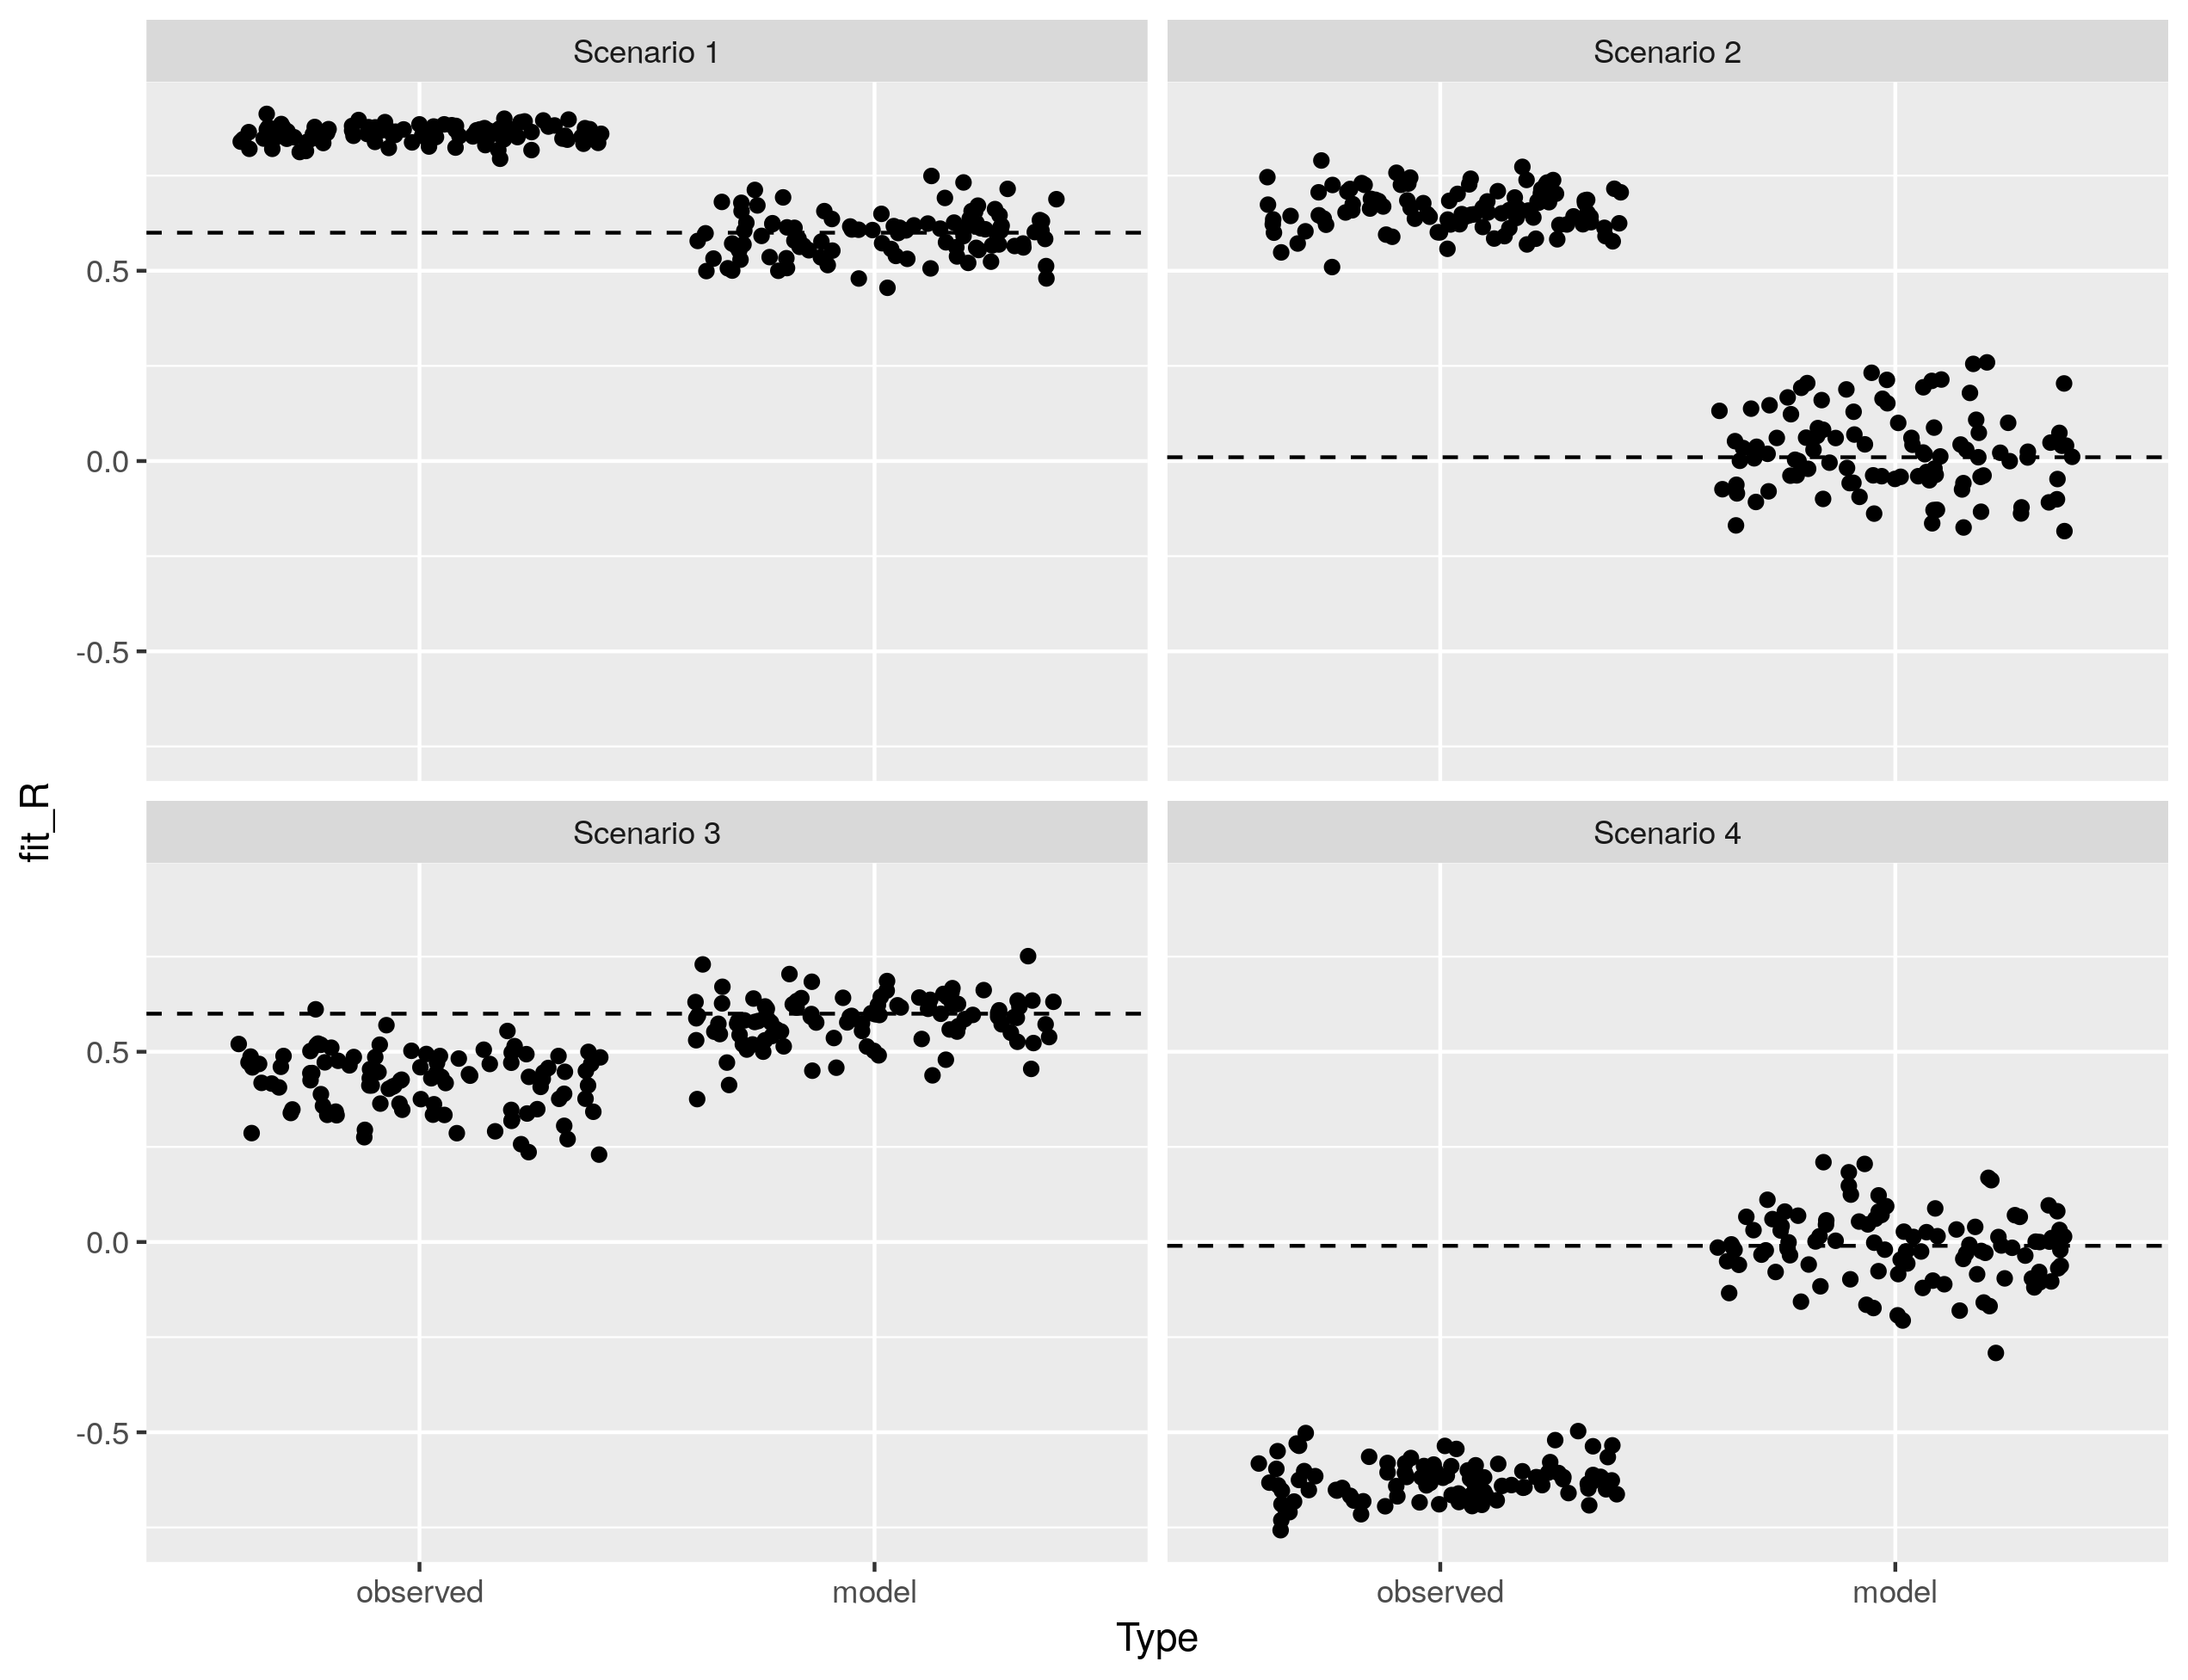
\includegraphics[width=\textwidth,keepaspectratio]{simulation1_4_res.png}
\end{figure}


\section*{Second simulations: two predictors, two responses}

In this second batch of simulations two predictors were generated, when these two predictors were included in the models the results are (as expected) the same as in the first round of simulation (ie: extrinsic correlation in the case of no residual correlation). More interesting is when one of the two predictor is dropped from the model based on the scenarios outlined in Table~\ref{tab:sim2}.

\begin{table}[h!]
\caption{Result second simulation round}
\label{tab:sim2}
 \begin{tabular}{lccr}
  Scenario ID & Predictor effect & Residual correlation & Result \\ \hline
  7 & divergent & no & Intrisic correlation \\
  8 & divergent & yes (positive) & Unresolved \\
  9 & consistent & yes (positive) & Intrisic correlation 
 \end{tabular}
\end{table}

In the case of a missing predictor with divergent effect between the response variables, even if the data were generated with no residual correlation, both the observed and the model residual will show some level of correlations due to the unaccounted-for effect of the second predictor (scenario 7). More complex is the case where there is divergent predictor effects plus residual correlation and one of the predictor is absent from the model. In that case depending on the strength of the effect and of the residual correlation there can be intrisic or extrinsic correlation being detected in the model residuals, sign changes are also likely to happen (scenario 8). Finally, when predictor have consistent effect, dropping a predictor from the model still leads to a correct detection of intrisic residual correlation (scenario 9). 


\end{document}
